\documentclass[a4paper,12pt,twocolumn]{article}
\usepackage{geometry}
\geometry{margin=0.5in}
\usepackage[utf8]{inputenc}
\usepackage[most]{tcolorbox}
\usepackage{chemmacros}
\usepackage{graphicx}
\usepackage[version=4]{mhchem}
\usepackage{nopageno}
\usepackage{tikz}

\newtcolorbox{Box1}[2][]{
                lower separated=false,
                colback=white!80!gray,
colframe=white, fonttitle=\bfseries,
colbacktitle=white!50!gray,
coltitle=black,
enhanced,
attach boxed title to top left={xshift=0.5cm,yshift=-2mm},
title=#2,#1}


\newtcolorbox{Box2}[2][]{
                lower separated=false,
                colback=white,
colframe=black,fonttitle=\bfseries,
colbacktitle=black,
coltitle=white,
enhanced,
attach boxed title to top left={yshift=-0.1in,xshift=0.15in},
                 boxed title style={boxrule=0pt,colframe=white,},
title=#2,#1}

\newtcolorbox{Box3}[2][]{
                lower separated=false,
                colback=white!80!gray,
colframe=white!20!black,fonttitle=\bfseries,
colbacktitle=white!30!gray,
coltitle=black,
enhanced,
attach boxed title to top left={xshift=0.5cm,
        yshift=-2mm},
title=#2,#1}

\newtcolorbox{Box4}[2][]{arc=0mm,
                lower separated=false,
                colback=white!80!gray,
colframe=white!20!black,fonttitle=\bfseries,
colbacktitle=white!30!gray,
coltitle=black,
enhanced,
attach boxed title to top left={xshift=0.5cm,
        yshift=-2mm},
title=#2,#1}

\newcommand{\oxi}[2]{%
    \stackrel{#1}{\mathrm{#2}}
}%
\DeclareUnicodeCharacter{2212}{-}

\begin{document}


\begin{center}
\huge{Oxidation And Reduction Reaction} \\[10pt]
\end{center}

\section{Oxidation-Reduction\\ Reactions}
\begin{itemize}
  \item \textbf{Oxidation-reduction} or \textbf{Redox}, reactions are considered electron transfer reactions.
  \item Oxidation-reduction reactions are very much a part of the world around us. They range from the burning of fossil fuels to the action of household bleach. 
  \item Most metallic and nonmetallic elements are obtained from their ores by the process of oxidation or reduction.
  \item Many important redox reactions take place in water, but not all redox reactions occur in aqueous solution.
\end{itemize}

\section{Oxidation-Reduction\\
and Half-Reactions}
\begin{itemize}
\item \textbf{Oxidation} is the loss of electrons from some chemical species, \textbf{Reduction} is the gain of electrons.
\item The species undergoing oxidation is referred to as a \textbf{reducing agent}.
\item The species undergoing reduction is referred to as an \textbf{oxidizing agent}.
\item \textbf{Oxidation:} an increase in the element’s oxidation number. 
\item \textbf{Reduction:} a decrease in oxidation number.
\end{itemize}

\begin{Box1}{}

$\stackrel{0}{\mathrm{Mg}}(s)+\stackrel{+1}{2 \mathrm{HCl}}(a q) \longrightarrow  \stackrel{+2}{\mathrm{MgCl}}_{2}(a q)+\stackrel{0}{\mathrm{H}}_{2}(g)$

\begin{itemize}
\item \textbf{Mg} metal is oxidized. Oxidation number increased from \textbf{0} to \textbf{+2}.
\item $\textbf{H}^+$ ions are reduced. Oxidation number reduced to \textbf{0} from \textbf{+1}.
\item $\textbf{Cl}^{-1}$ is spectator ions.
\end{itemize}
\end{Box1}

\begin{figure}[h]
\centering
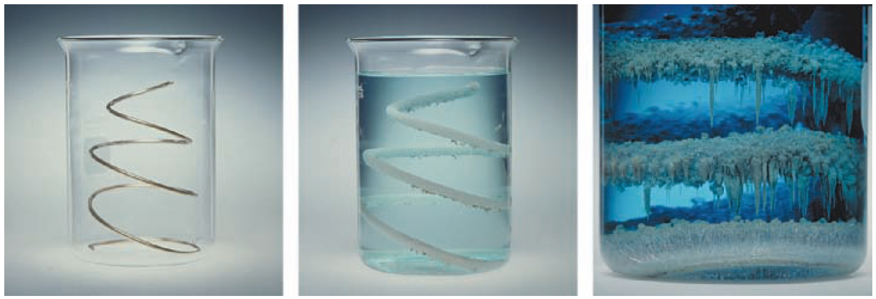
\includegraphics[width=0.5\textwidth]{cupper.png}
\end{figure}
\begin{center}
A clean copper wire is placed into a colorless solution of silver nitrate
\end{center}


$\begin{array}{cc}
\mathrm{Cu}(\mathrm{s}) \rightarrow \mathrm{Cu}^{2+}(\mathrm{aq})+2 \mathrm{e}^{-} & \text {Oxidation Half-reaction } \\
2 \mathrm{Ag}^{+}(\mathrm{aq})+2 \mathrm{e}^{-} \rightarrow 2 \mathrm{Ag}(\mathrm{s}) & \text { Reduction Half-reaction }
\end{array}$
\newline
\begin{Box2}{Example}
\begin{center}
$\ce{2Mg + O2 -> 2MgO}$
\end{center}
Magnesium oxide (MgO) is an ionic compound made up of $\ce{Mg^{2+}}$ and $\ce{O^{2-}}$ ions. In
this reaction, two $\ce{Mg}$ atoms give up or transfer four electrons to two O atoms (in $\ce{O2}$ ).
For convenience, we can think of this process as two separate steps, one involving
the loss of four electrons by the two Mg atoms and the other being the gain of four
electrons by an $\ce{O2}$ molecule:
\begin{center}
$\ce{2Mg -> 2Mg^{2+} + 4e^-}$\\
$\ce{O2 + 4e^- -> 2O^{2-}}$
\end{center}
Each of these steps is called a \textbf{half-reaction}, which explicitly shows the electrons
involved in a redox reaction. The sum of the half-reactions gives the overall reaction:
\begin{center}
$\ce{2Mg + O2 + 4e^- ->  2O^{2-} + 2Mg^{2+} + 4e^-}$
\end{center}
or, if we cancel the electrons that appear on both sides of the equation,
\begin{center}
$\ce{2Mg + O2 ->  2O^{2-} + 2Mg^{2+}}$
\end{center}
Fially, the $\ce{O^{2-} and Mg^{2+}}$ ions combine to form $\ce{MgO}$:
\begin{center}
$\ce{2Mg^{2+} + 2O^{2-} -> 2MgO}$
\end{center}
\end{Box2}
\begin{itemize}
\item An \textbf{oxidation reaction} refers to the half-reaction that involves loss of electrons.
\item A \textbf{reduction reaction} is a half-reaction that involves gain of electrons.
\item In the formation of magnesium oxide, magnesium is oxidized. It is said to act as a reducing agent because it donates electrons to oxygen and causes oxygen to be reduced. Oxygen is reduced and acts as an oxidizing agent because it accepts electrons from magnesium, causing magnesium to be oxidized. 
\item The extent of oxidation in a redox reaction must be equal to the extent of reduction; that is, the number of electrons lost by a reducing agent must be equal to the number of electrons gained by an oxidizing agent.

\end{itemize}

\begin{Box2}{Example}\begin{center}
$\ce{Zn + CuSO4 -> ZnSO4 + Cu}$
\end{center}
In the process, the solution loses the blue color that characterizes the presence of hydrated $\ce{Cu^{2+}}$:
\begin{center}
$\ce{Zn + Cu^{2+} -> Zn^{2+} + Cu}$
\end{center}
The oxidation and reduction half-reactions are:
\begin{center}
$\ce{Zn -> Zn^{2+} + 2e^-}$\\
$\ce{Cu^{2+} + 2e^- -> Cu}$
\end{center}
Similarly, metallic copper reduces silver ions in a solution of silver nitrate ($\ce{AgNO3}$):
\begin{center}
$\ce{Cu(s) + 2AgNO3(aq) -> Cu(NO3)2(aq) + 2Ag(s)}$
\end{center}
\end{Box2}
\section{Oxidation Number}
Oxidation number of an atom, also called the oxidation state, signifies the number of charges the atom would have in a molecule (or an ionic compound) if electrons were transferred completely.
\begin{center}
$\stackrel{0}{\mathrm{Mg}}(s)+\stackrel{+1}{2 \mathrm{HCl}}(a q) \longrightarrow  \stackrel{+2}{\mathrm{MgCl}}_{2}(a q)+\stackrel{0}{\mathrm{H}}_{2}(g)$
\end{center}
\begin{enumerate}
\item In free elements (that is, in the uncombined state), each atom has an oxidation number of zero. Thus, each atom in $\ce{H2, Br2, Na, Be, K, O2}$, and $\ce{P4}$ has the same oxidation number: zero.
\item For ions composed of only one atom (that is, monatomic ions), the oxidation number is equal to the charge on the ion. Thus, Li ion has an oxidation number of +1; $\ce{Ba^{2+}}$ ion, +2; $\ce{Fe^{3+}}$ ion, +3; $\ce{I^{-}}$ ion, −1; $\ce{O^{2-}}$ ion, −2; and so on. All alkali metals have an oxidation number of +1 and all alkaline earth metals have an oxidation number of +2 in their compounds. Aluminum has an oxidation number of +3 in all its compounds.
\item The oxidation number of oxygen in most compounds (for example, $\ce{MgO}$ and $\ce{H2O}$) is −2, but in hydrogen peroxide ($\ce{H2O2}$) and peroxide ion ($\ce{O^{2-}}$), it is −1.
\item The oxidation number of hydrogen is +1, except when it is bonded to metals in binary compounds. In these cases (for example, $\ce{LiH, NaH, CaH2}$), its oxidation number is -1.
\item Fluorine has an oxidation number of −1 in all its compounds.Other halogens (Cl, Br, and I) have negative oxidation numbers when they occur as halide ions in their compounds. When combined with oxygen-for example in oxoacids and oxoanions. They have positive oxidation numbers.
\item In a neutral molecule, the sum of the oxidation numbers of all the atoms must be zero. In a polyatomic ion, the sum of oxidation numbers of all the elements in the ion must be equal to the net charge of the ion. For example, in the ammo- nium ion, $\ce{NH^{4+}}$, the oxidation number of N is -3 and that of H is +1. Thus the sum of the oxidation numbers is −3 + 4(+1) = +1, which is equal to the net charge of the ion.
\item Oxidation numbers do not have to be integers. For example, the oxidation number of O in the superoxide ion, $\ce{O^{-}2}$, is $-\dfrac{1}{2}$.
\end{enumerate}

\section{Types of Redox Reactions}
\subsection{Combination Reaction}
A \textbf{combination reaction} is a reaction in which two or more substances combine to form a single product. 
\begin{Box1}{}
$\stackrel{0}{\mathrm{S}}(s)+\stackrel{0}{\mathrm{O_2}}(g) \longrightarrow  {\mathrm{\stackrel{+4}{S}\stackrel{-2}{O}_2}}(g)$\\
$\stackrel{0}{2 \mathrm{Al}}(s)+\stackrel{0}{3\mathrm{Br_2}}(l) \longrightarrow  {2\mathrm{\stackrel{+3}{Al}\stackrel{-1}{Br}_3}}(s)$
\end{Box1}
\begin{figure}[h]
\centering
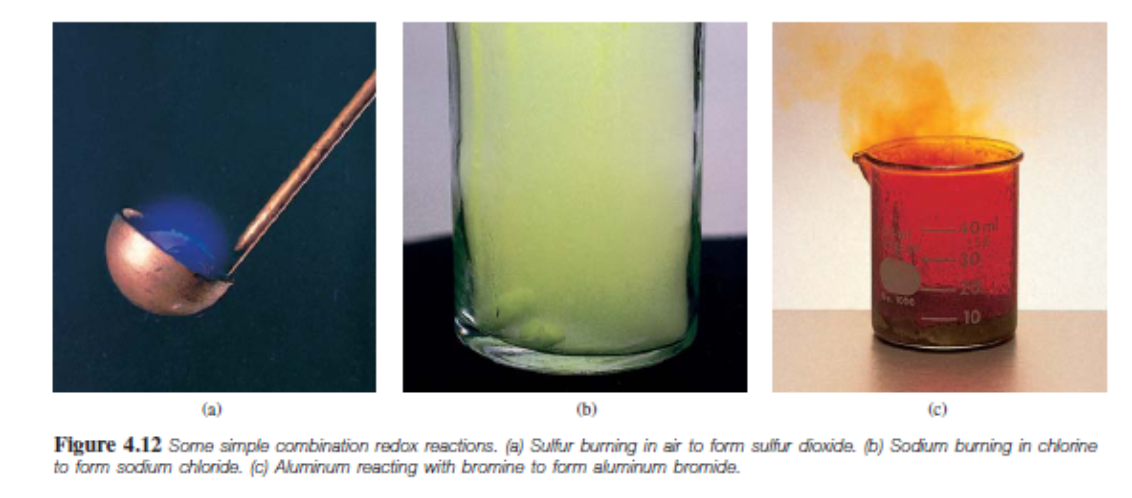
\includegraphics[width=0.5\textwidth, height=1.1in]{combination.png}
\end{figure}
\newpage
\subsection{Decomposition Reaction}
\begin{itemize}
\item \textbf{Decomposition reactions} are the opposite of \textbf{combination reactions}. 
\item Specifically, a \textbf{decomposition reaction} is the breakdown of a compound into two or more components. 
\end{itemize}
\begin{Box1}{}
${2\mathrm{\stackrel{+2}{Hg}\stackrel{-2}{O}_2}}(s) \longrightarrow   \stackrel{0}{2\mathrm{Hg}}(l)+\stackrel{0}{\mathrm{O_2}}(g) $\\
${2\mathrm{\stackrel{}{K}\stackrel{+5}{Cl}\stackrel{-2}{O}_3}}(s) \longrightarrow   \stackrel{}{2\mathrm{K}}\stackrel{-1}{\mathrm{Cl}}(s)+\stackrel{0}{3\mathrm{O_2}}(g) $\\
${2\mathrm{\stackrel{+1}{Na}\stackrel{-1}{H}}}(s) \longrightarrow   \stackrel{0}{2\mathrm{Na}}(s)+\stackrel{0}{3\mathrm{H_2}}(g) $
\end{Box1}

\begin{figure}[h]
\centering
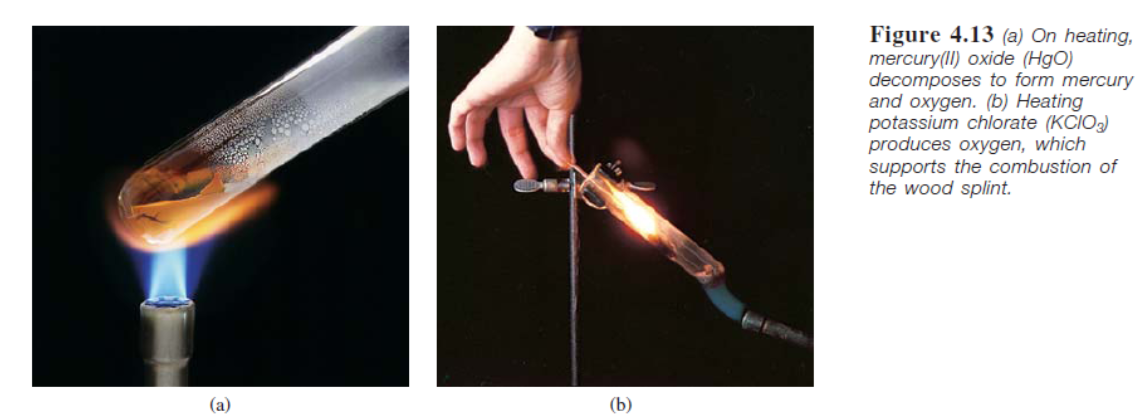
\includegraphics[width=0.5\textwidth]{decomposition.png}
\end{figure}

\subsection{Combustion Reaction}
\begin{itemize}
\item \textbf{Combustion} reaction is a reaction in which a substance reacts with \textbf{oxygen}, usually with the release of heat and light to produce a flame. 
\item The reactions between magnesium and sulfur with oxygen are combustion reactions.
\item The burning of propane ($\mathrm{C_3H_8}$), a component of natural gas that is used for domestic heating and cooking, is also a combustion reaction.:
\begin{Box1}{}
$\mathrm{C}_{3} \mathrm{H}_{8}(g)+5 \mathrm{O}_{2}(g) \longrightarrow 3 \mathrm{CO}_{2}(g)+4 \mathrm{H}_{2} \mathrm{O}(l)$
\end{Box1}
\item Assigning an oxidation number to C atoms in organic compounds is more involved. Here, we focus only on the oxidation number of O atoms, which changes from 0 to 2.
\\
\\
\end{itemize}

\subsection{Displacement Reactions}
\begin{itemize}
\item In a \textbf{displacement reaction}, an ion (or atom) in a compound is replaced by an ion (or atom) of another element.
\item Most displacement reactions fit into one of three subcategories:
      \begin{enumerate}
      \item \textbf{Hydrogen Displacement}
      \item \textbf{Metal Displacement}
      \item \textbf{Halogen Displacement}

      \end{enumerate}
\end{itemize}
\subsubsection{Hydrogen Displacement}
\begin{itemize}
  \item All alkali metals and some alkaline earth metals (Ca, Sr, and Ba), which are the most reactive of the metallic elements, will displace hydrogen from cold water.
\end{itemize}
\begin{Box1}{}
$\ce{2Na(s) + 2H2O(l) -> 2NaOH(aq) + H2(g)}$\\
$\ce{Ca(s) + 2H2O(l) -> Ca(OH)2(s) + H2(g)}$
\end{Box1}
\begin{figure}[h]
\centering
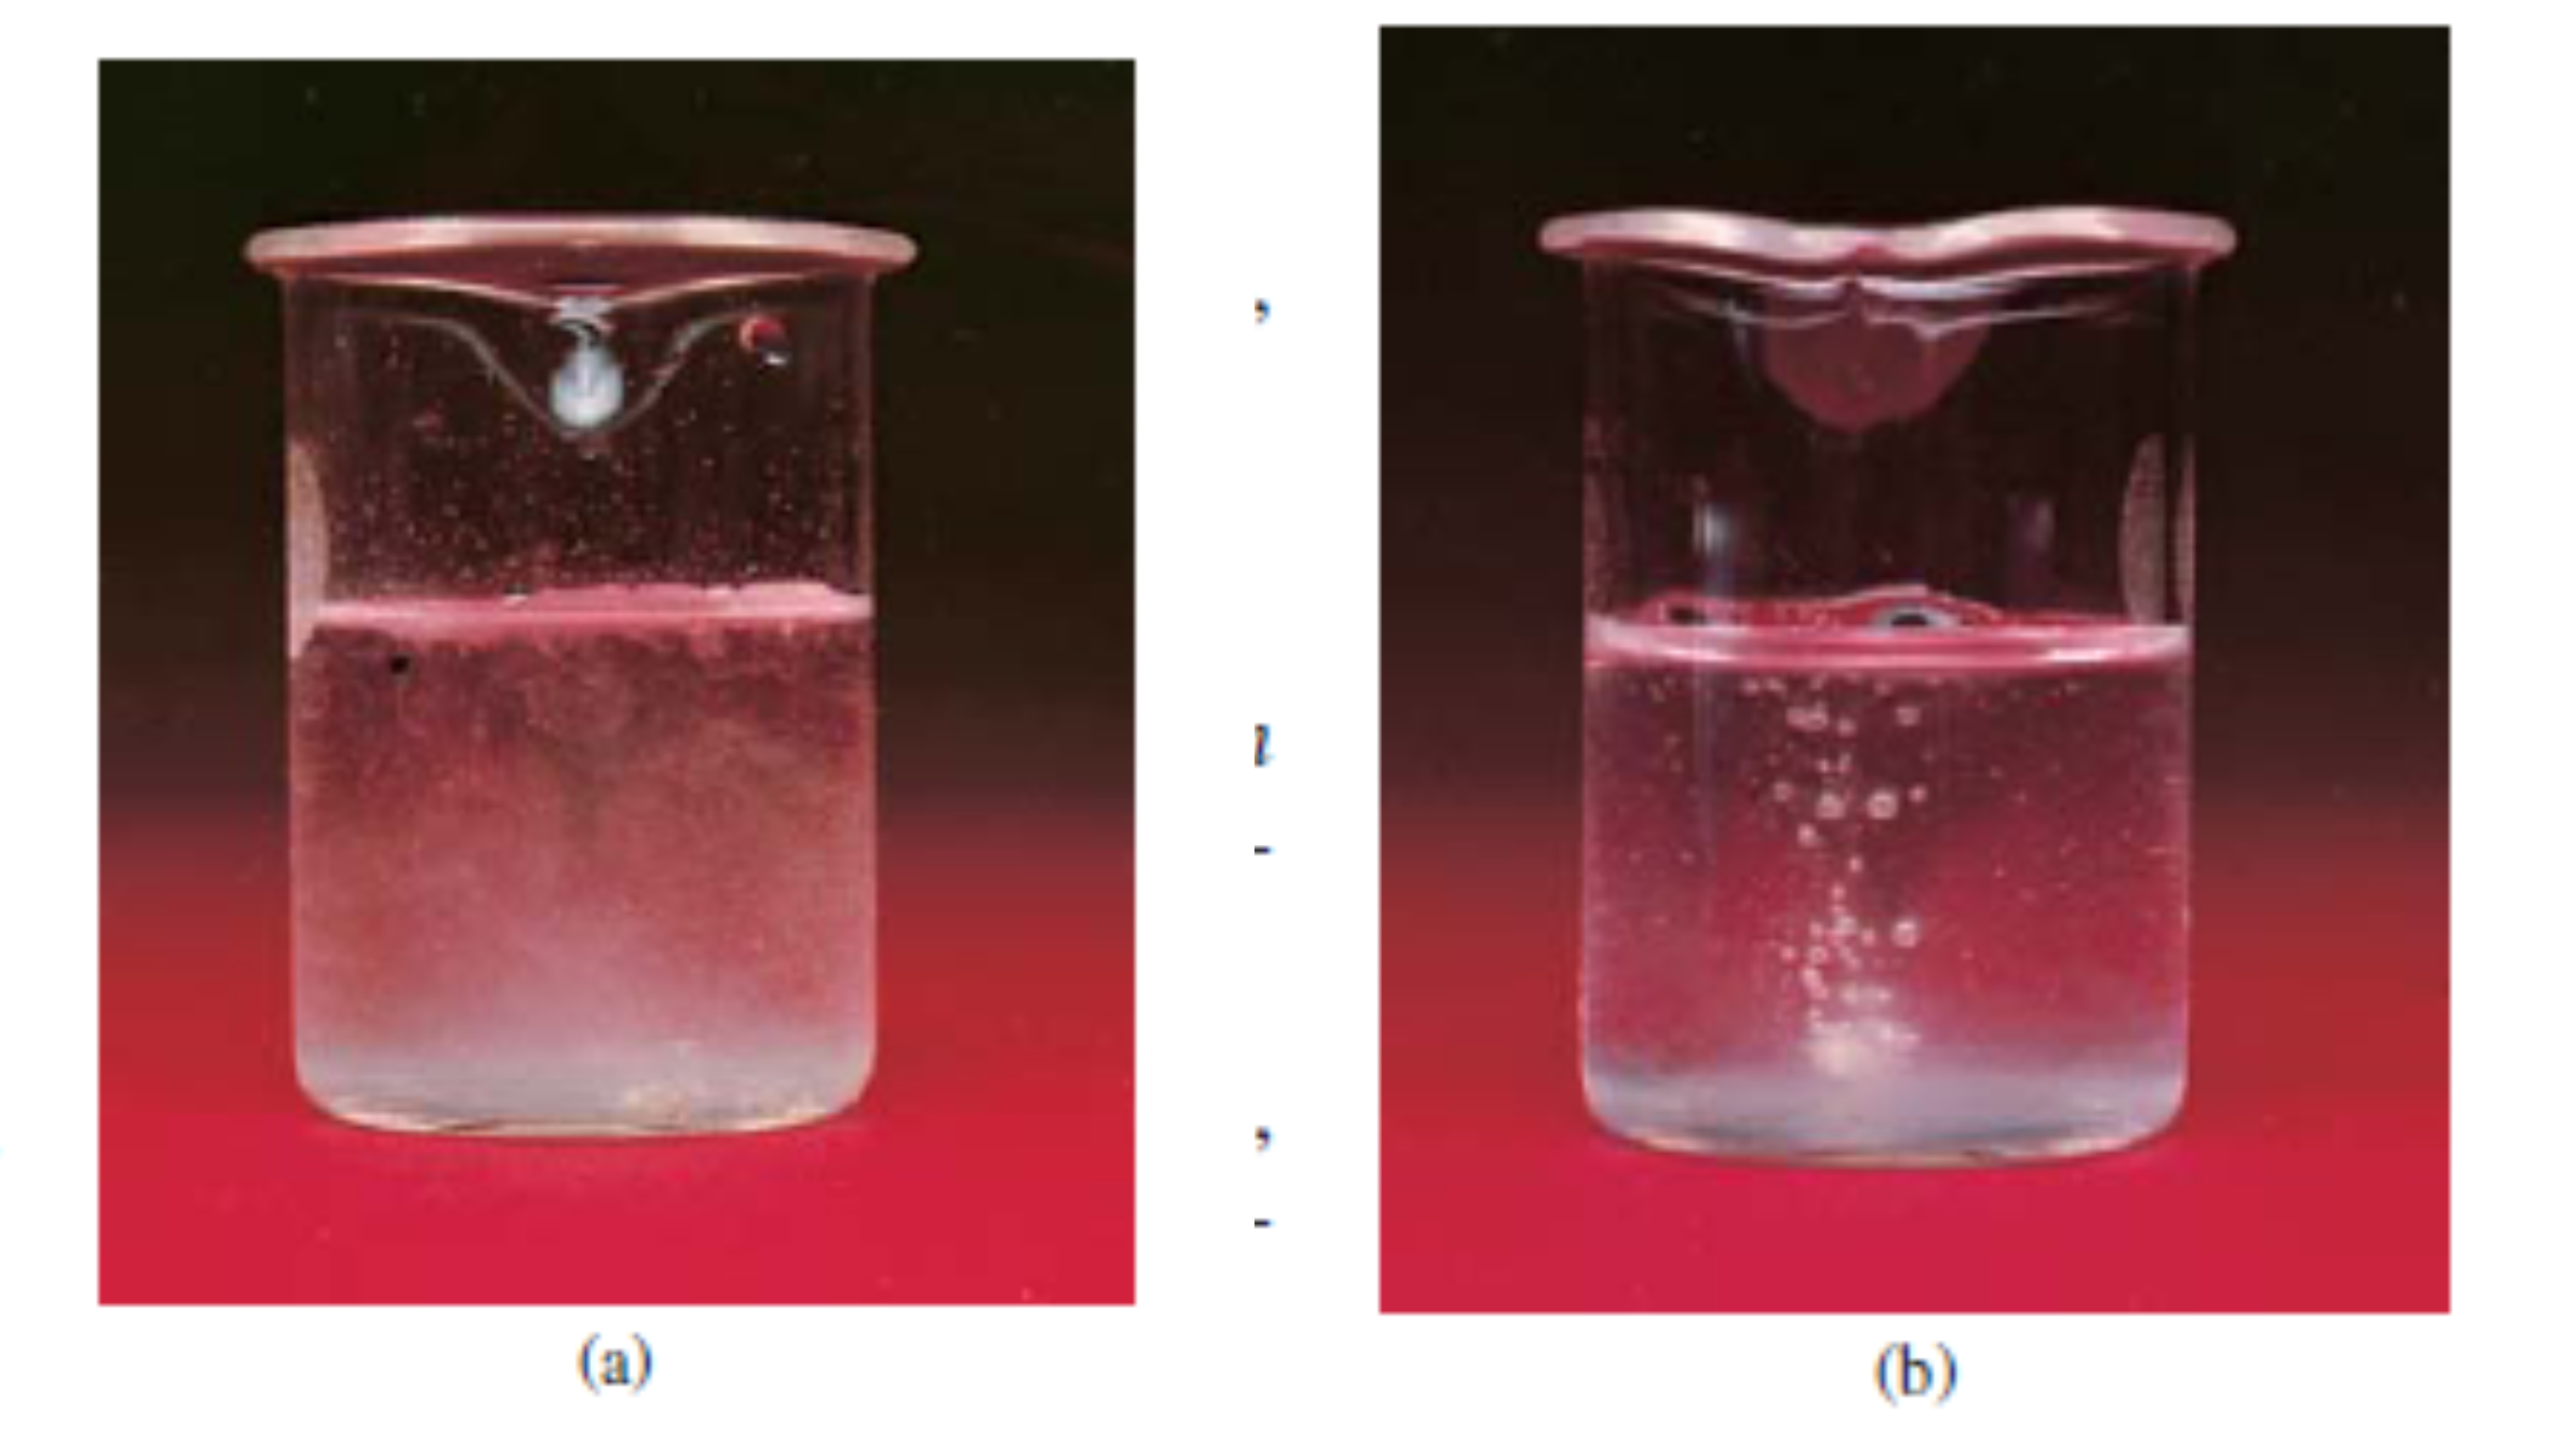
\includegraphics[width=0.5\textwidth]{hydrogen.png}
\end{figure}
\begin{itemize}
  \item Many metals, including those that do not react with water, are capable of displacing hydrogen from acids. For example, zinc (Zn) and magnesium (Mg) do not react with cold water but do react with hydrochloric acid, as follows:
\end{itemize}
\begin{Box1}{}
$\ce{Zn(s) + 2HCl(aq) -> ZnCl2(aq) + H2(g)}$\\
$\ce{Mg(s) + 2HCl(aq) -> MgCl2(aq) + H2(g)}$
\end{Box1}
\begin{figure}[h]
\centering
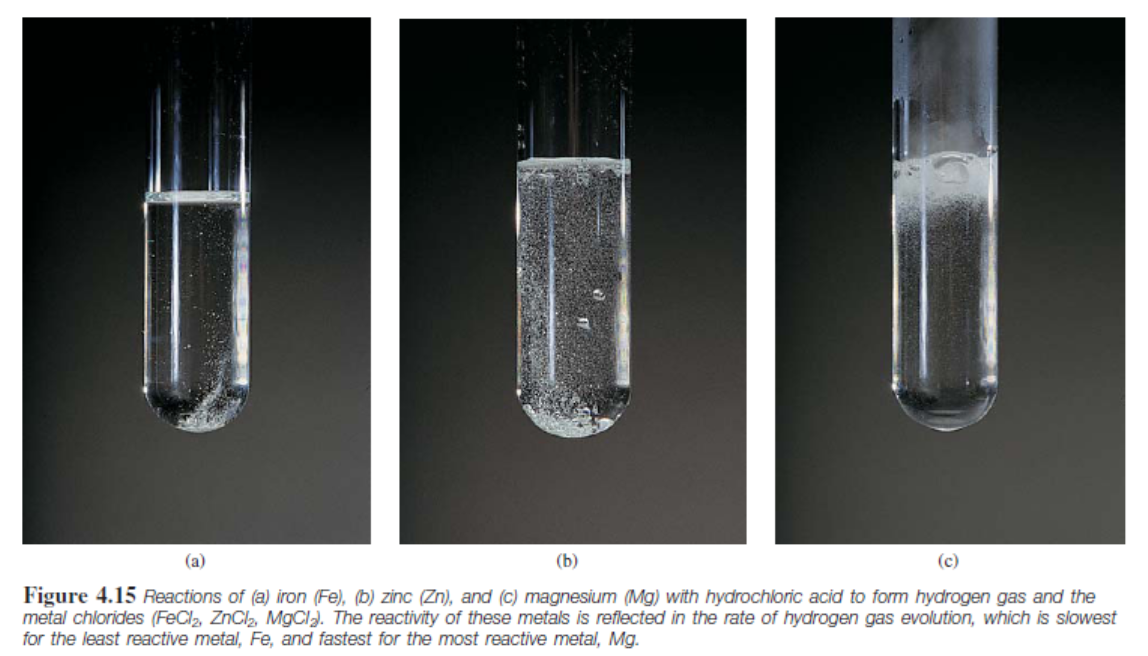
\includegraphics[width=0.5\textwidth]{hydrogen1.png}
\end{figure}
\subsubsection{Metal Displacement}
\begin{itemize}
\item A metal in a compound can be displaced by another metal in the elemental state. 
\item For example, zinc replaces copper ions and copper replaces silver ions. 
\item Reversing the roles of the metals would result in no reaction. Thus, copper metal will not displace zinc ions from zinc sulfate, and silver metal will not displace copper ions from copper nitrate.
\item An easy way to predict whether a metal or hydrogen displacement reaction will actually occur is to refer to an \textbf{activity series (the electrochemical series)}. 
\item Basically, an activity series is a \textbf{convenient summary of the results of many possible displacement reactions.}
\item According to this series, any metal above hydrogen will displace it from water or from an acid, but metals below hydrogen will not react with either water or an acid. In fact, any metal listed in the series will react with any metal (in a compound) below it. For example, Zn is above Cu, so zinc metal will displace copper ions from copper sulfate.
\end{itemize}
\begin{figure}[h]
\centering
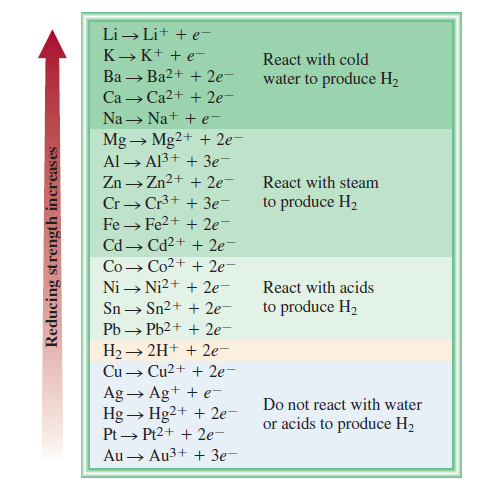
\includegraphics[width=3.5in]{activity.png}
\end{figure}

\begin{itemize}
\item Metal displacement reactions find many applications in metallurgical processes,
the goal of which is to separate pure metals from their ores. For example, vanadium
is obtained by treating vanadium(V) oxide with metallic calcium.
Similarly, titanium is obtained from titanium(IV) chloride.
\end{itemize}
\begin{Box1}{}
$\ce{V2O5 + 5Ca -> 2V + 5CaO}$\\
$\ce{TiCl4 + 2Mg -> Ti + 2MgCl2}$
\end{Box1}
\subsubsection{Halogen Displacement}
\begin{Box1}{}
\begin{center}
$\ce{F2} > \ce{Cl2} > \ce{Br2} > \ce{I2}$
\end{center}
\end{Box1}
The power of these elements as oxidizing agents decreases as we move down Group
7A from fl uorine to iodine, so molecular fl uorine can replace chloride, bromide, and
iodide ions in solution. In fact, molecular fl uorine is so reactive that it also attacks
water; thus these reactions cannot be carried out in aqueous solutions. On the other
hand, molecular chlorine can displace bromide and iodide ions in aqueous solution.
The displacement equations are:
\begin{Box1}{}
$\ce{Cl2 + 2KBr -> 2KCl + Br2}$\\
$\ce{Cl2 + 2NaI -> 2NaCl + I2}$
\end{Box1}
The ionic equations are:
\begin{Box1}{}
$\ce{Cl2 + 2Br^{-} -> 2Cl^{-} + Br2}$\\
$\ce{Cl2 + 2I^{-} -> 2Cl^{-} + I2}$
\end{Box1}
Molecular bromine, in turn, can displace iodide ion in solution:
\begin{Box1}{}
$\ce{Br2 + 2I^{-} -> 2Br^{-} + I2}$
\end{Box1}
Reversing the roles of the halogens produces no reaction. Thus, bromine cannot displace
chloride ions, and iodine cannot displace bromide and chloride ions.
\subsection{Disproportionation Reaction}
\begin{itemize}
\item In a \textbf{disproportionation reaction}, an element in one oxidation state is simultaneously oxidized and reduced.
\item One reactant in a disproportionation reaction always contains an element that can have at least three oxidation states. The element itself is in an intermediate oxidation state; that is, both higher and lower oxidation states exist for that element in the products.

\begin{Box1}{}
$\ce{2H2O2 -> 2H2O + O2}$
\end{Box1}
Here the oxidation number of oxygen in the reactant (-1) both increases to zero in
$\ce{O2}$ and decreases to -2 in $\ce{H2O}$. Another example is the reaction between molecular chlorine and $\ce{NaOH}$ solution:
\begin{Box1}{}
$\mathrm{Cl}_{2}(g)+2 \mathrm{OH}^{-}(a q) \longrightarrow \mathrm{ClO}^{-}(a q)+\mathrm{Cl}^{-}(a q)+\mathrm{H}_{2} \mathrm{O}(l)$
\end{Box1}
\end{itemize}
\begin{Box1}{Example}
$\small{\begin{array}{l}\text{(a) } 2 \mathrm{~N}_{2} \mathrm{O} \longrightarrow 2 \mathrm{~N}_{2}+\mathrm{O}_{2}\\
\text{(b) } 6 \mathrm{Li}+\mathrm{N}_{2} \longrightarrow 2 \mathrm{Li}_{3} \mathrm{N}\\
\text{(c) } \mathrm{Ni}+\mathrm{Pb}\left(\mathrm{NO}_{3}\right)_{2} \longrightarrow  \mathrm{Pb}+\mathrm{Ni}\left(\mathrm{NO}_{3}\right)_{2}\\
\text{(d) } 2 \mathrm{NO}_{2}+\mathrm{H}_{2} \mathrm{O}(l) \longrightarrow  \mathrm{HNO}_{2}+\mathrm{HNO}_{3}
\end{array}}$
\end{Box1}

\begin{Box2}{Solution}
(a) This is a decomposition reaction because one reactant is converted to two
different products. The oxidation number of N changes from +1 to 0, while that of
O changes from +2 to 0.\\
\\
(b) This is a combination reaction (two reactants form a single product). The oxidation
number of Li changes from 0 to +1 while that of N changes from 0 to +3.\\
\\
(c) This is a metal displacement reaction. The Ni metal replaces (reduces) the Pb ion.
The oxidation number of Ni increases from 0 to +2 while that of Pb decreases
from +2 to 0.\\
\\
(d) The oxidation number of N is +4 in $\ce{NO2}$ and it is +3 in $\ce{HNO2}$ and +5 in $\ce{HNO3}$.
Because the oxidation number of the same element both increases and decreases,
this is a disproportionation reaction.
\end{Box2}

\subsection{Breathalyzer}
\begin{figure}[h]
\centering
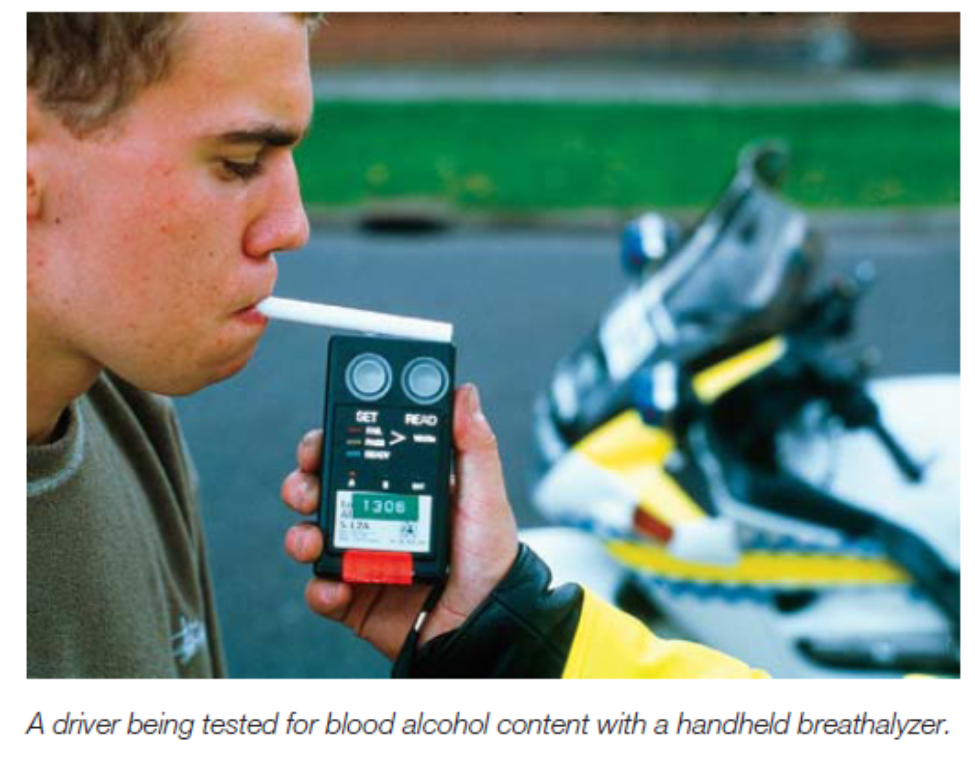
\includegraphics[width=0.5\textwidth]{breathalyzer.png}
\end{figure}
\begin{itemize}
\item The police often use a device called a breathalyzer to test drivers suspected of being drunk. 
\item The chemical basis of this device is a redox reaction. A sample of the driver’s breath is drawn into the breathalyzer, where it is treated with an acidic solution of potassium dichromate. 
\item The alcohol (ethanol) in the breath is converted to acetic acid as shown in the following equation:\\
\end{itemize}

\begin{Box1}{}
$\ce{3CH3CH2OH + 2K2Cr2O7 + 8H2SO4 -> 3CH3COOH + 2Cr2(SO4)3 + 2K2SO4 + 11H2O}$
\end{Box1}
\begin{itemize}
\item In this reaction, the ethanol is oxidized to acetic acid and the chromium(VI) in the orange-yellow dichromate ion is reduced to the green chromium(III) ion. 
\item The driver’s blood alcohol level can be determined readily by measuring the degree of this color change (read from a calibrated meter on the instrument). 
\item The current legal limit of blood alcohol content in most states is 0.1 percent by mass. Anything higher constitutes intoxication.

\end{itemize}

\subsection{Balancing Redox Equations}
\subsubsection{Acidic Medium}
{\large Balancing the equation showing the oxidation of $\ce{Fe^{2+}}$ ions to $\ce{Fe^{3+}}$ ions by dichromate ions $\ce{Cr2O^{2-}7}$ in an acidic medium.}
\begin{enumerate}
\item Write the unbalanced equation for the reaction in ionic form.
\begin{center}
$\ce{Fe^{2+} + Cr2O^{2-}7 -> Fe^{3+} + Cr^{3+}}$
\end{center}
\item Separate the equation into two half reactions.\\
\begin{center}
Oxidation: $\ce{Fe^{2+} -> Fe^{3+}}$\\
Reduction: $\ce{Cr2O^{2-}7 -> Cr^{3+}}$
\end{center}
\item Balance each half-reaction for number and type of atoms and charges. For reactions in an acidic medium, add $\ce{H2O}$ to balance the O atoms and $\ce{H^+}$ to balance the H atoms.\\
\\
\\
\textbf{Oxidation half-reaction:} The atoms are already balanced. To balance the charge, we add an electron to the right hand side of the arrow:
    \begin{center}
        $\ce{Fe^{2+} -> Fe^{3+} + e^-}$
    \end{center}
    \textbf{Reduction half-reaction:} Because the reaction takes place in an acidic medium, we add seven $\ce{H2O}$ molecules to the right hand side of the arrow to balance the O atoms:
    \begin{center}
    $\ce{Cr2O^{2-}7 -> Cr^{3+} + 7H2O}$
    \end{center}
    To balance the H atoms, we add $\ce{14H^+}$ ions on the left-hand side:\
    \begin{center}
    $\ce{14H^+ + Cr2O^{2-}7 -> Cr^{3+} + 7H2O}$
    \end{center}
    There are now 12 positive charges on the left-hand side and only six positive charge on the right hand side. Therefore, we add six electrons on the left:
    \begin{center}
     $\ce{14H^+ + Cr2O^{2-}7 + 6e^- -> Cr^{3+} + 7H2O}$
    \end{center}
    \item Add the two half-equations together and balance the final equation by inspection. The electrons on both sides must cancel. If the oxidation and reduction half-reactions contain different numbers of electrons, we need to multiply one or both half-reactions to equalize the number of electrons.
    \\
    \begin{center}
    $\ce{6( Fe^{2+} -> Fe^{3+} + e^- )}$\\
    $\ce{14H^+ + Cr2O^{2-}7 + 6e^- -> Cr^{3+} + 7H2O}$
    \line(1,0){240}\\
    $\ce{Fe^{2+} + 14H^+ + Cr2O^{2-}7 + 6e^- -> 6Fe^{3+} + Cr^{3+} + 7H2O + 6e^-}$
    \end{center}
    The electrons on both sides cancel, and we are left with the balanced net ionic equations:
    \begin{center}
        $\ce{Fe^{2+} + 14H^+ + Cr2O^{2-}7 -> 6Fe^{3+} + Cr^{3+} + 7H2O}$
    \end{center}
    \item Verify that the equation contains the same type and numbers of atoms and the same charges on both sides of the equation.
    A final check shows that the resulting  equation is "atomically" and "electrically balanced".
\end{enumerate}
\subsubsection{Basic Medium}
{\large Write a balanced ionic equation to represent the oxidation of iodine ion ($\ce{I^-}$) by permangante ion ($\ce{MnO^{-}4}$) in basic solution to yield molecular iodine ($\ce{I2}$)and manganese(IV) oxide ($\ce{MnO2}$)}.
\begin{enumerate}
\item The unbalanced equation is:
\begin{center}
$\mathrm{MnO}_{4}^{-}+\mathrm{I}^{-} \longrightarrow \mathrm{MnO}_{2}+\mathrm{I}_{2}$
\end{center}
\item The two half-reactions are:
\begin{center}
Oxidation: $\mathrm{I}^{-} \longrightarrow \mathrm{I}_{2}$\\
Reduction: $\mathrm{MnO}_{4}^{-} \longrightarrow \mathrm{MnO}_{2}$
\end{center}
\item We balance each half-reaction for number and type of atoms and charges.\\
\\
\textbf{Oxidation half-reaction:} We first balance the I atoms:
\begin{center}
$2 \mathrm{I}^{-} \longrightarrow \mathrm{I}_{2}$
\end{center}
To balance charges, we add two electrons to the right-hand side of the equations:
\begin{center}
$2 \mathrm{I}^{-} \longrightarrow \mathrm{I}_{2}+2 e^{-}$
\end{center}
\textbf{Reduction half-reaction:} To balance the O atoms, we add two $\ce{H2O}$ molecules on the right:
\begin{center}
$\mathrm{MnO}_{4}^{-} \longrightarrow \mathrm{MnO}_{2}+2 \mathrm{H}_{2} \mathrm{O}$
\end{center}
To balance the H atoms, we add four $\ce{H^+}$ ions son the left: 
\begin{center}
$\mathrm{MnO}_{4}^{-}+4 \mathrm{H}^{+} \longrightarrow \mathrm{MnO}_{2}+2 \mathrm{H}_{2} \mathrm{O}$
\end{center}
There are three net positive charges on the left, so we add three electrons to the same side to balance the charges:
\begin{center}
$\mathrm{MnO}_{4}^{-}+4 \mathrm{H}^{+}+3 e^{-} \longrightarrow \mathrm{MnO}_{2}+2 \mathrm{H}_{2} \mathrm{O}$
\end{center}
\item We now add the oxidation and reduction half reactions to give the overall reaction. In order to equalize the number of electrons, we need to multiply the oxidation half-reaction by 3 and the reduction half-reaction by 2 as follows: \\

\begin{center}
$3\left(2 \mathrm{I}^{-}\right.  \left.\longrightarrow \mathrm{I}_{2}+2 e^{-}\right)$ \\
$2\left(\mathrm{MnO}_{4}^{-}+4 \mathrm{H}^{+}+3 e^{-}\right.  \left.\longrightarrow \mathrm{MnO}_{2}+2 \mathrm{H}_{2} \mathrm{O}\right)$ \\
 $\line(1,0){240}$\\
$6 \mathrm{I}^{-}+2 \mathrm{MnO}_{4}^{-}+8 \mathrm{H}^{+}+6 e^{-}  \longrightarrow 3 \mathrm{I}_{2}+2 \mathrm{MnO}_{2}+4 \mathrm{H}_{2} \mathrm{O}+6 e^{-}$
\end{center}

The electrons on both sides cancel and we are left with the balanced net ionic equation: 
\begin{center}
$6 \mathrm{I}^{-}+2 \mathrm{MnO}_{4}^{-}+8 \mathrm{H}^{+} \longrightarrow 3 \mathrm{I}_{2}+2 \mathrm{MnO}_{2}+4 \mathrm{H}_{2} \mathrm{O}$
\end{center}
This is balanced equation in acidic medium. However, because the reaction is carried out in a basic medium, for every $\ce{H^+}$ ion we need to add equal number of $\ce{OH^-}$ ions to both sides of the equations:
\begin{center}
$6 \mathrm{I}^{-}+2 \mathrm{MnO}_{4}^{-}+8 \mathrm{H}^{+}+8 \mathrm{OH}^{-} \longrightarrow 3 \mathrm{I}_{2}+2 \mathrm{MnO}_{2}+4 \mathrm{H}_{2} \mathrm{O}+8 \mathrm{OH}^{-}$
\end{center}
Finally, combining the  $\ce{H^+}$ and  $\ce{OH^-}$ ions to form water, we obtain:
\begin{center}
$6 \mathrm{I}^{-}+2 \mathrm{MnO}_{4}^{-}+4 \mathrm{H}_{2} \mathrm{O} \longrightarrow 3 \mathrm{I}_{2}+2 \mathrm{MnO}_{2}+8 \mathrm{OH}^{-}$
\end{center}
\item A final check shows that the resulting  equation is "atomically" and "electrically balanced".
\end{enumerate}

\end{document}